% !TeX root = ../thuthesis-example.tex

\chapter{技术方案}
\section{点线联合网络SP-SOLD2}
\subsection{网络设计}
为了构建可以联合推理点线特征及其描述子的网络,首先需要考察同时进行点/线提取和描述的神经网络。为了寻找最合适的点/线神经网络方法,我们对目前的点特征神经网络进行了基准测试,测试了各类点特征网络和匹配方法在Hpatches数据集上的匹配精度和运行时间,测试结果如表\ref{tab_PLtest}所示。
\begin{table}[!ht]
  \centering
  \begin{tabular}{|c|c|c|c|c|c|c|c|}
  \hline
      Algorithm & Train Set & \makecell{MMA\\@1} & \makecell{MMA\\@3} & \makecell{MMA\\@5} & \makecell{Time Cost\\(ms)} & Features & Matches \\ \hline
      \parbox[c][9ex]{2cm}{LoFTR} &  \parbox[c][9ex]{3.5cm}{ResNet18 backbone + MegaDepth (309K)} & 0.47 & 0.76 & 0.81 & 210 & 7397 & 7397 \\ \hline
      \parbox[c][13ex]{2cm}{Patch2Pix (with SuperGlue)} & \parbox[c][9ex]{3.5cm}{ResNet34 backbone + MegaDepth (309K)} & 0.43 & 0.81 & 0.90 & <426 & 1233 & 1233 \\ \hline
      \parbox[c][9ex]{2cm}{Patch2Pix} & \parbox[c][9ex]{3.5cm}{ResNet34 backbone + MegaDepth (309K)} & 0.34 & 0.66 & 0.74 & 707 & 1994 & 1994 \\ \hline
      \parbox[c][9ex]{2cm}{SuperPoint + SuperGlue} & \parbox[c][9ex]{3.5cm}{SuperPoint:MS-COCO 2014 (83K)} & 0.36 & 0.76 & 0.88 & 94 & 2002 & 1233 \\ \hline
      \parbox[c][9ex]{2cm}{ASLFeat + NN} & \parbox[c][9ex]{3.5cm}{GL3D (125K)} & 0.4 & 0.72 & 0.82 & 263 & 3924 & 1993 \\ \hline
      \parbox[c][9ex]{2cm}{R2D2 + NN} & \parbox[c][17ex]{3.5cm}{Random Web images + Aachen DB images + Aachen style transfer pairs + Aachen optical flow pairs (16K)} & 0.34 & 0.67 & 0.74 & 67 & 3568 & 1133 \\ \hline
      \parbox[c][9ex]{2cm}{R2D2(单通道) + NN} & \parbox[c][17ex]{3.5cm}{Random Web images + Aachen DB images + Aachen style transfer pairs + Aachen optical flow pairs (16K)} & 0.34 & 0.67 & 0.74 & 67 & 3332 & 1148 \\ \hline
      \parbox[c][9ex]{2cm}{SuperPoint + NN} & \parbox[c][9ex]{3.5cm}{MS-COCO 2014 (83K)} & 0.33 & 0.64 & 0.74 & 29 & 2002 & 1082 \\ \hline
      \parbox[c][9ex]{2cm}{R2D2(MS) + NN} & \parbox[c][17ex]{3.5cm}{Random Web images + Aachen DB images + Aachen style transfer pairs + Aachen optical flow pairs (16K)} & 0.32 & 0.74 & 0.83 & 179 & 4894 & 1685 \\ \hline
      \parbox[c][9ex]{2cm}{D2-Net\\+ NN} &  \parbox[c][9ex]{3.5cm}{VGG16 backbone + MegaDepth (309K)} & 0.11 & 0.43 & 0.67 & 976 & 6414 & 2495 \\ \hline
      \parbox[c][9ex]{2cm}{ORB +\\ BFMatch} & $\backslash$ & 0.256 & 0.491 & 0.543 & 93 & 4436 & 1603 \\ \hline
  \end{tabular}
  \caption{点特征神经网络测试结果}
  \label{tab_PLtest}
\end{table}

根据第一章节的调研结果和此处的测试结果,综合考虑实时性和精度效果,最终选取了Superpoint\cite{detone2018superpoint}点特征网络和SOLD2\cite{pautrat2021sold2}线特征网络进行联合设计。Superpoint网络由一个共享编码网络(Shared Encoder),一个特征点解码网络(Interest Point Decoder)和一个特征点描述网络(Descriptor Decoder)组成;而SOLD2网络由一个共享骨干编码网络(Shared Backbone Encoder)和三个解码网络组成,三个解码网络分别负责推理线端点概率图(Junction Map),线概率图(Line Heatmap)和线描述子特征图(Descriptor map)。对比发现,Superpoint中的特征点解码网络和SOLD2中的线端点概率图解码网络有类似的卷积层和相似的功能(提取感兴趣的点);此外在SOLD2一文中,线特征的描述子来自于对线上点的抽样。结合这两个观察,我们将两个网络的骨干编码网络和特征点、描述子解码网络进行合并,得到了点线联合网络SP-SOLD2,如图\ref{fig_sp_sold}。
\begin{figure}
  \centering
  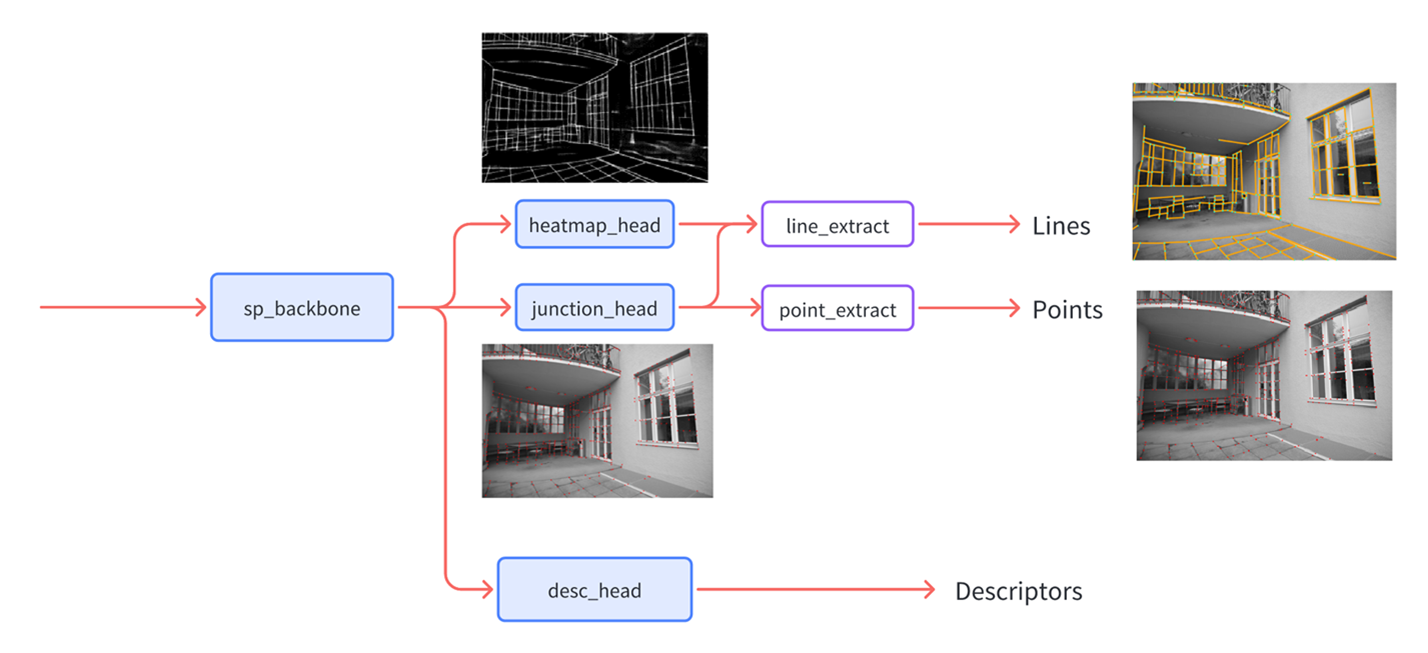
\includegraphics[width = 0.85\textwidth]{sp_sold.png}
  \caption{SP-SOLD2网络结构示意图}
  \label{fig_sp_sold}
\end{figure}

在SP-SOLD2网络中,输入图像(尺寸为$[H, W]$)首先会经过一个含有四个block的骨干编码网络(每个block含有两个卷积层和一个最大池化层,最后一个块没有池化层),得到一个尺寸为$[H/8, W/8, 128]$的特征图;这一特征图会经过不同的卷积解码器得到与原图尺寸一致的两个概率图$\mathcal{H}$和$\mathcal{J}$,以及一个尺寸为$[H/8, W/8, 128]$的描述子特征图$\mathcal{D}$。

为了从概率图得到图像中的点/线提取结果,需要对$\mathcal{H}$和$\mathcal{J}$进行后处理,具体步骤如下:
\begin{enumerate}
  \item 对概率图$\mathcal{J}$进行softmax和nms操作,并经过阈值筛选得到特征点提取结果。
  \item 利用不同的阈值,同理可以从概率图$\mathcal{J}$中获得线端点的候选集合$J$。
  \item 利用三角筛选法对线端点进行初筛:任意连接两个端点,去除掉以连线为中垂线的三角形内其余端点,更新集合$J$。这一步的目的是去除“杂点”,避免最后得到的线段过于密集。
  \item 对概率图$\mathcal{H}$进行sigmoid操作得到$\mathcal{H'}$,并以此计算候选端点连线的得分:对于$J$中的任意两个端点连线,根据$\mathcal{H'}$获取连线上每个像素某半径范围内的平均概率值作为线段得分。
  \item 根据线段得分和线段上采样点得分数组进行筛选得到线段提取结果:要求是线段得分大于阈值且线段采样点得分大于阈值超过一定比例。
\end{enumerate}
为了从描述子特征图$\mathcal{D}$得到点和线段对应的描述子,需要对其进行插值和采样操作;其中,线特征的描述子由一系列采样点组成,如果将采样点数目超参定义为N,则每条线段的描述子维度是[N, 128]。

\subsection{网络训练}
在训练中,损失函数包含三个部分:前两个分支的概率图$\mathcal{H}$和$\mathcal{J}$的损失,以及第三个分支的描述子对于点/线参数化的损失。参考两篇文章\cite{detone2018superpoint}\cite{pautrat2021sold2},我们对于三个损失函数的定义如下:
\begin{enumerate}
  \item 概率图$\mathcal{H}$对应的$\hat{\mathbf{H}}\left(I ; f_{\text {heat }}\right)$(其中$\mathcal{H_i}$表示单应变换)
  \[\begin{aligned}
    \hat{\mathbf{H}}\left(I ; f_{\text {heat }}\right) & =\frac{1}{N_{h}} \sum_{i=1}^{N_{h}} \mathcal{H}_{i}^{-1}\left(f_{\text {heat }}\left(\mathcal{H}_{i}(I)\right)\right)
    \end{aligned}\]
  \item 概率图$\mathcal{J}$对应的$\hat{\mathbf{J}}\left(I ; f_{\text {junc }}\right)$
  \[\begin{aligned}
    \hat{\mathbf{J}}\left(I ; f_{\text {junc }}\right) & =\frac{1}{N_{h}} \sum_{i=1}^{N_{h}} \mathcal{H}_{i}^{-1}\left(f_{\text {junc }}\left(\mathcal{H}_{i}(I)\right)\right)
    \end{aligned}\]
  \item 描述子特征图$\mathcal{D}$对应的:
  \[
  \mathcal{L}_{desc}=w_l*\frac{1}{n}\sum^n_{i=1}
  max(0,M+p_i-n_i)+w_p*\frac{1}{\left(H_{c} W_{c}\right)^{2}} \sum_{\substack{h=1 \\
  w=1}}^{H_{c}, W_{c}} \sum_{\substack{h^{\prime}=1 \\
  w^{\prime}=1}}^{H_{c}, W_{c}} l_{d}\left(\mathbf{d}_{h w}, \mathbf{d}_{h^{\prime} w^{\prime}}^{\prime} ; s_{h w h^{\prime} w^{\prime}}\right)
  \]
  where
  \[
  p_i=||D_1^i-D_2^i||_2, n_i=min(||D_I^i-D_2^{h_2(i)}||_2,||D_1^{h_1(i)}-D_2^i||_2), h_1(i)=argmin_{k\in[1,n]}||D_i^k-D_2^i||
  \]
  \[\begin{aligned}
  l_{d}\left(\mathbf{d}, \mathbf{d}^{\prime} ; s\right)&=\lambda_{d} * s * \max \left(0, m_{p}-\mathbf{d}^{T} \mathbf{d}^{\prime}\right)+(1-s) * \max \left(0, \mathbf{d}^{T} \mathbf{d}^{\prime}-m_{n}\right)\\
  s_{hwh'w'}&=\begin{cases}1,&\text{if}||\widehat{\mathcal{H}\mathbf{p}_{hw}}-\mathbf{p}_{h'w'}||\le8\\0,&\text{otherwise}\end{cases}\\
  \end{aligned}\]
\end{enumerate}
描述子的损失函数可以理解为点/线描述子的损失函数加权和,前半部分为线描述子的损失函数,利用已知单应变换的匹配点对,将在两张图中属于同一线段的点对和不属于同一线段但距离小于阈值的点对作triple loss;后半部分为点描述子的损失函数,用整个cell作为匹配单元(认为相同cell内的点在单应变换前后都匹配),利用一对cell描述子$d_{hw}\in D$和$d'_{h'w'}\in D'$,建立一个单应变换关系的判据$s_{hwh'w'}$,构造hingle loss。于是,联合损失函数被定义为:
\[
  \begin{aligned}\mathcal{L}_{total}&=e^{-w_{junc}}\mathcal{L}_{junc}+e^{-w_{line}}\mathcal{L}_{line}+e^{-w_{desc}}\mathcal{L}_{desc}+w_{junc}+w_{line}+w_{desc}\end{aligned}
\]
为了训练这一点线联合网络,本工作基于两篇文章的思路,继续构建了一个完整的自监督训练流程:
\begin{enumerate}
  \item 利用简单数据集Synthetic对网络进行预训练,只训练点/线提取的两个分支,得到预训练网络;
  \item 从训练集中获取图片$I$,并进行单应变换得到四个变换图$I_1, I_2, I_3, I_4$;
  \item 利用预训练网络对四个单应图片进行点线特征提取,并对提取到的点和线段进行反单应变换作为原图的点线特征真值;
  \item 利用真值,在训练集上继续调优预训练网络,使得网络在训练集上具有提取点/线特征的能力;
  \item 解冻描述子分支,对整个网络进行训练,在训练中调整各损失函数的比重以加快收敛,最终得到可以一次推理出点线特征及其描述子的联合网络模型。
\end{enumerate}

\section{前端自定义点线VIO框架NN-PL-VIO}
本工作基于ROS节点构建的PL-VINS框架,修改构建了一个支持神经网络的前端自定义的点线VIO框架NN-PL-VIO。PL-VINS框架有相对清晰完整的节点划分,便于进行修改,并且其工作面向实时性目标展开,符合本课题的实时性要求。
\begin{figure}
  \centering
  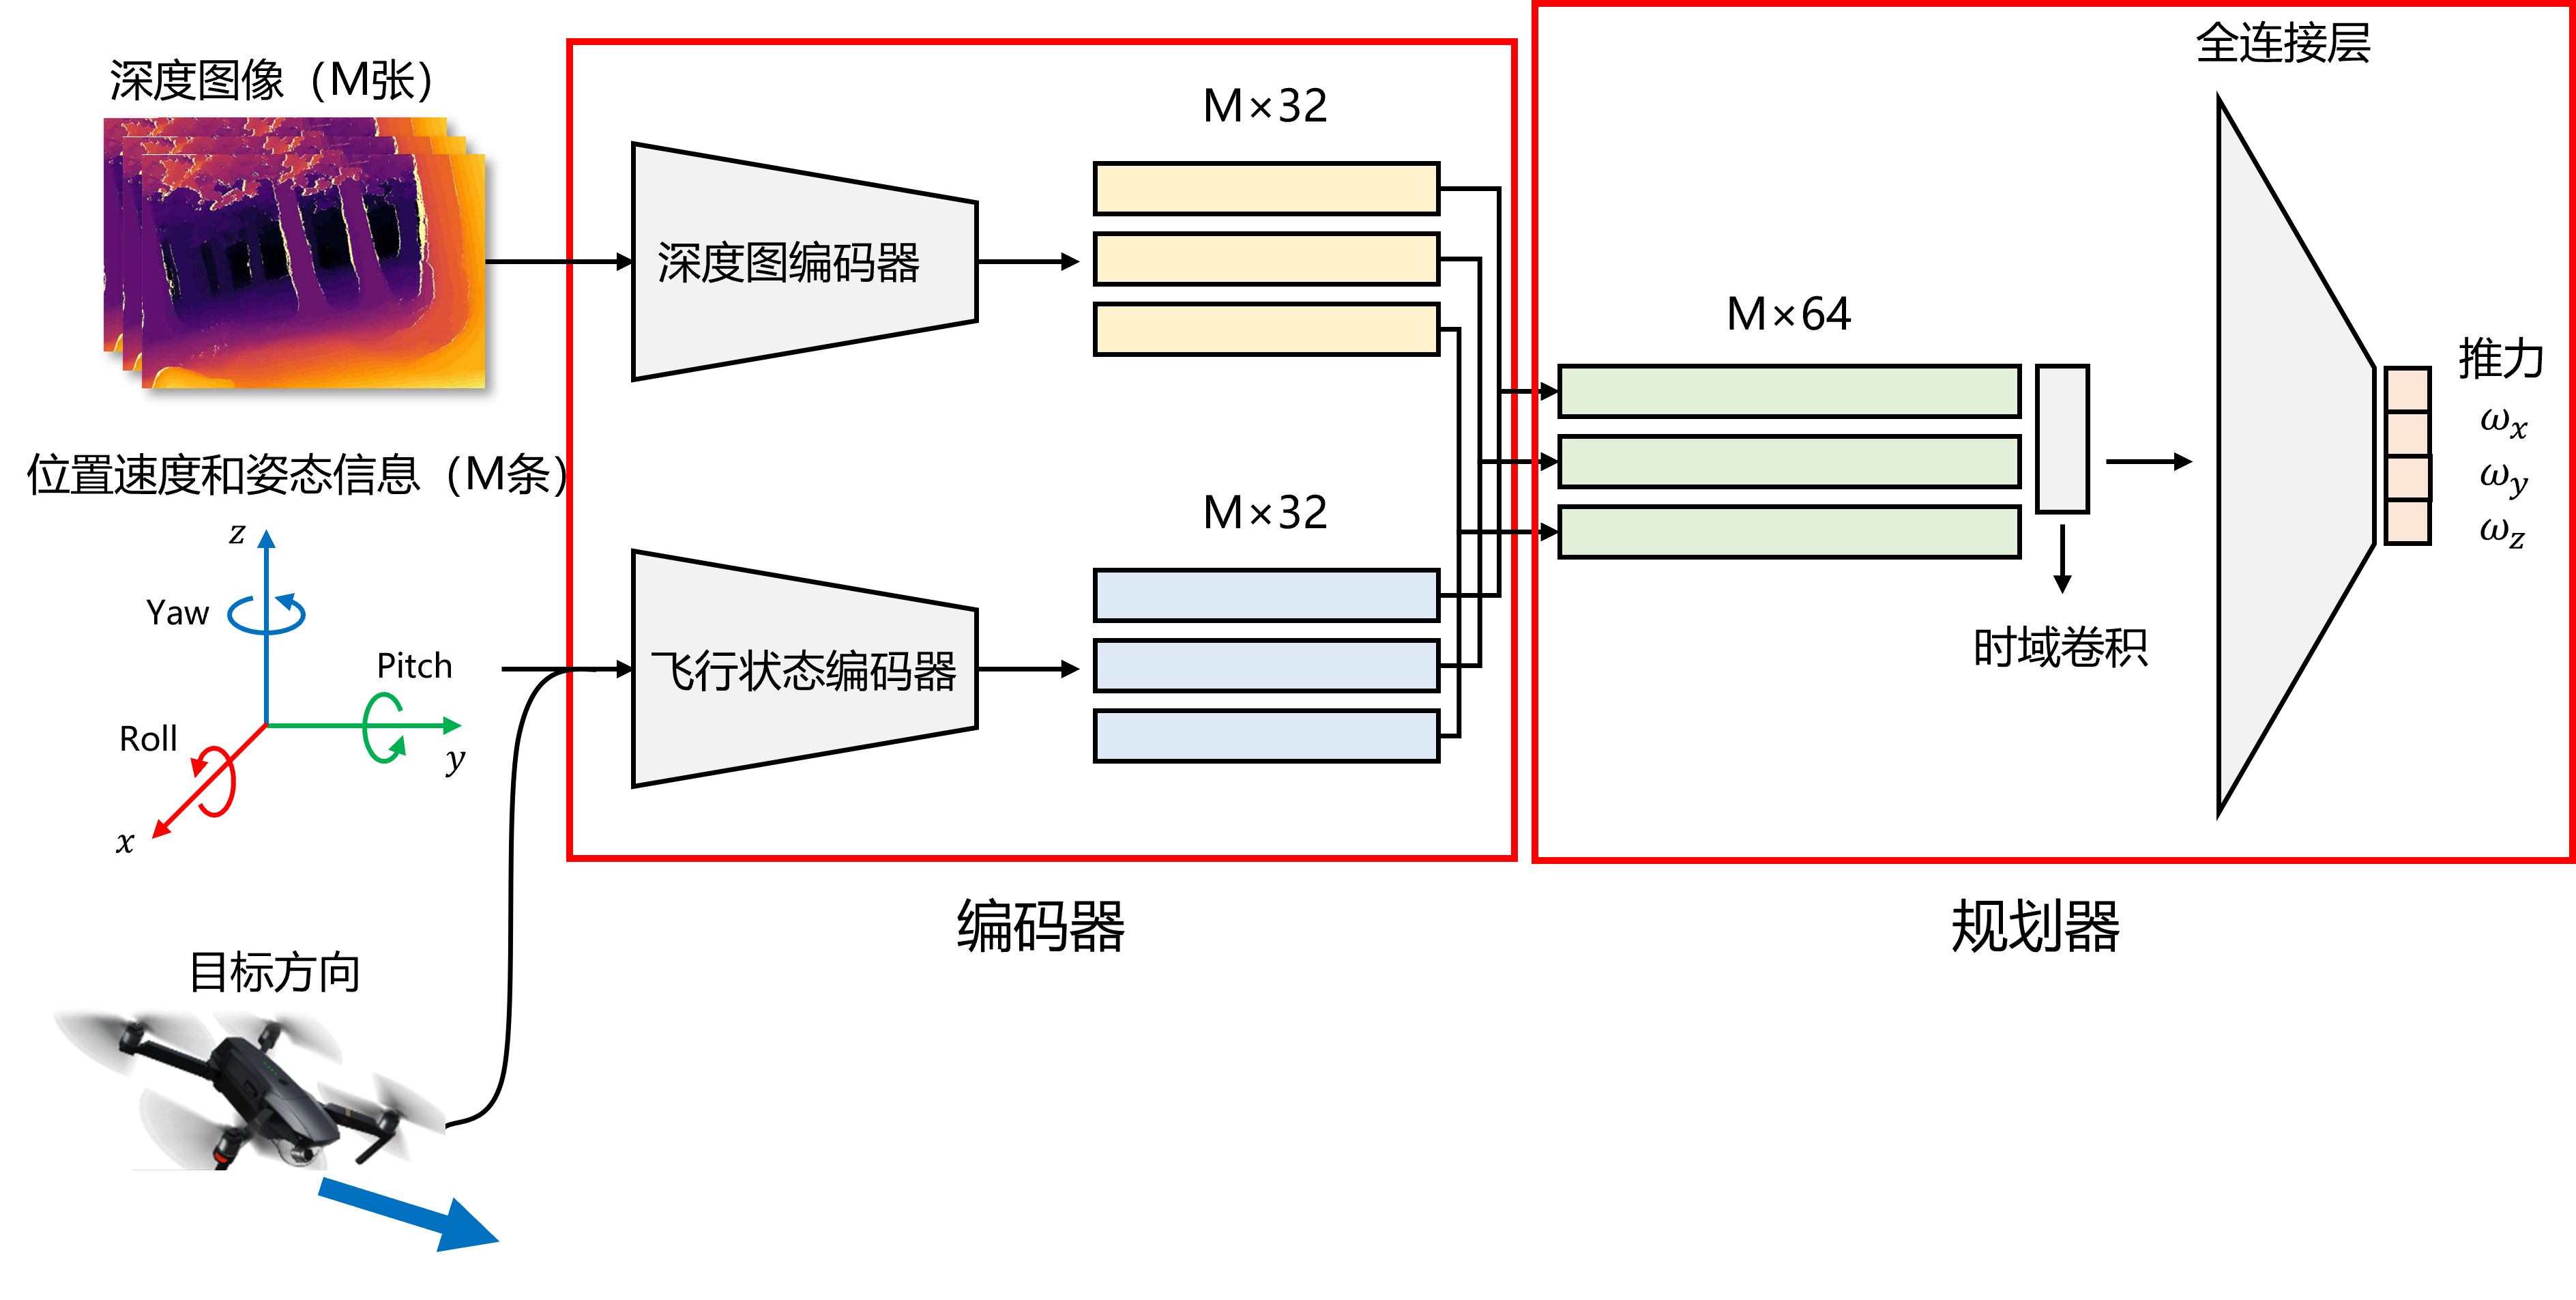
\includegraphics[width = 0.9\textwidth]{framework.png}
  \caption{前端自定义点线VIO框架NN-PL-VIO}
  \label{fig_framework}
\end{figure}
PL-VINS框架中含有四个节点,分别是点特征处理节点、线特征处理节点、位姿轨迹估计节点和回环检测节点。其中,点/线特征处理节点负责持续接收图像输入,提取图像中的点线特征并完成帧间特征匹配;位姿轨迹估计节点负责接收匹配结果和IMU读数,利用优化方法进行位姿估计和轨迹重建;而回环检测节点使用图像中的点特征和关键帧检测相机是否经过了相同的场景地点,并以此纠正累计误差,提高重建轨迹的精度。

\section{速度优化}
为了在嵌入式设备上实时运行整个框架,本工作对于最为耗时的点线神经网络后处理部分进行了速度优化。
\subsection{SoftMax优化}
在SP-SOLD2网络的点特征后处理部分,本工作合并了SoftMax和NMS(非极大值抑制,Non-Maximum Suppression)操作,并利用置信度最大点减小了计算量。

由于最终筛选的特征点数量远小于图像网格数量,因此我们只选择8x8网格区域内置信度最高的点进行除法操作。原始的Softmax操作可以表示为:
\[\sigma(\mathbf{z})_i=\frac{e^{z_i}}{\sum_{j=0}^Ke^{z_j}},i=1,\ldots,K\]
其中$\sigma(\mathbf{z})_i$表示原始图像区域中的 8x8 区域中的第 i 个点的置信度。因此,对于优化前的算法,每次 Softmax 操作计算需要除法运算次数为:
\[
  \#SoftDiv_{ori}=H_{c}\times W_{c}\times 65
\]
在大多数情况下,因为选取的特征点数量 k 远小于网格数量$H_c\times W_c$, 而 Softmax 使得每个网格区域的置信度之和为1,因此只有在每个 8x8 网格区域中置信度最高的点可能在排序后被选中。只在网格区域中置信度最大点执行 Softmax 操作可以减小存储和计算开销,并简化后续计算的复杂性。因此,我们只计算 8x8 区域中最大元素的相应 Softmax 结果。找出 z 中最大元素,并假设第 m 个元素为最大元素,最大元素记为$\mathrm{z_m}$,只需计算$\mathrm{z_m}$相应的 Softmax 计算结果,它只消耗 1 次除法运算:
\[
  \sigma(\mathbf{z})_m=\frac{e^{z_m}}{\sum_{j=0}^Ke^{z_j}}
\]
Softmax 优化后共需要计算的除法次数:
\[\#SoftDiv_{opt}=H_c\times W_c\times1\]
通过这种稀疏化的Softmax操作,本方法将除法运算量大幅减少了。

对于同样耗时的非极大值抑制(NMS)操作,由于上一步的稀疏化 Softmax 计算已经抑制了特征点周围的部分像素,因此我们只需要每个 8x8 块内的特征点的最近邻居进行非极大值抑制即可。具体来说,NMS 首先假定有效候选特征点为图像中全部像素的集合, 然后对于原始输入图像的每个像素,NMS 将该像素的置信度与周围距离小于$\varepsilon_\mathrm{ori}$的区域中的像素的置信度进行比较。如果中心目标像素的置信度不是此区域中的最大值, 则该点将从有效候选特征点集合中删除。NMS 的输出是全部有效候选特征点的坐标和其置信度组成的列表。

在原始的后处理算法中,一般使用切比雪夫距离来度量像素间距离,即对于点$p( x_1, y_1)$和点$p(x_2,y_2)$, 它们的距离定义为:
\[dist(p_1,p_2)=\lim_{t\to\infty}(|x_1-x_2|^t+|y_1-y_2|^t)^{\frac1t}=max\:(|x_1-x_2|,|y_1-y_2|)\]
\begin{figure}
  \centering
  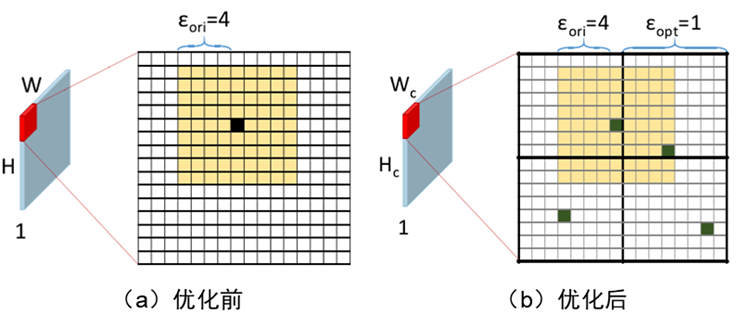
\includegraphics[width = 0.75\textwidth]{nms.png}
  \caption{优化前后非极大值抑制示意图}
  \label{fig_nms}
\end{figure}
因此,对于图中所示的原始输入图像中的每个像素(如图\ref{fig_nms},黑色), NMS 将该像素与周围边长为$(2\varepsilon_\mathrm{ori}+1)$的正方形区域(黄色)中的像素的置信度进行比较。在优化之前,每个像素包含H x W个像素,NMS 对每个像素进行$((2\varepsilon_\mathrm{ori}+1)^2-1)$次比较操作(不需要与自身进行比较)。因此,在原始 NMS 方法中,共需要的比较次数为:
\[\#NMSComp_{ori}=H\times W\times((2\varepsilon_{ori}+1)^2-1)\]
我们引入针对 Softmax 的优化给出了每个 8x8 网格区域中的最大置信度的像素, 与之相邻的网格区域中也仅有最大置信度的像素。如图中 (b) 所示,每个网格区域中的最大置信度标记为绿色。我们在网格的维度进行 NMS 操作,对于原始输入图像中的每个网格区域中的最大置信度的像素,NMS 将比较该网格的置信度与周围距离小于等于$\varepsilon_\mathrm{opt}$的每个网格区域内的最大置信度进行比较($\varepsilon_\mathrm{opt}$是网格的距离而非像素的距离), 并且删除极大值点。此处的距离不再以像素数为单位,而是以网格数为单位。因此$\varepsilon_\mathrm{opt}$和$\varepsilon_\mathrm{ori}$的关系可以表示为:
\[\varepsilon_{opt}=\left\lceil\frac{\varepsilon_{ori}}{8}\right\rceil\]
优化后,每个像素包含$H_{\mathrm{c}}\times W_{\mathrm{c}}$个网格区域,NMS 对每个网格区域进行$((2\varepsilon_\mathrm{opt}+1)^2-1)$次比较操作,共需要的比较操作次数为:
\[\#NMSComp_{opt}=H_c\times W_c\times\left(\left(2\varepsilon_{opt}+1\right)^2-1\right)\]
在实际实现中,$\varepsilon_{\mathrm{ori}}=4$, 因此
\[\#NMSComp_{opt}=H_c\times W_c\times((2\times1+1)^2-1)=H_c\times W_c\times8\]
可以看到优化后,NMS 所需要的比较操作次数减少了640倍。

\subsection{三角化初筛优化}
对于SP-SOLD2网络的线特征后处理部分,去除了耗时较高的三角化初筛方法,并采用更简单的双线性搜索来提取线段。在三角化初筛中,为了去除相隔较近的线端点,会计算所有线段两两内积(以此得到线段夹角和位置关系),在这一操作中,对于N个线段端点候选点,其计算复杂度为
\[O(\frac{C^2_N(C^2_N-1)}{2})=O(N^4)\]
根据实验结果,这将占据后处理30\%的时间。鉴于网络应用于VIO框架中,可以牺牲一部分线段提取准确度换取实时性能,故而在速度优化中选择去除三角化初筛,并且降低线端点的候选点数,以此达到控制线端点候选点数量的目的同时尽可能减小计算量。在利用线端点候选点和概率图提取线段的过程中,原方法采用了步骤较多的局部最大值搜索算法。这一算法会对所有线段进行采样并计算采样点一定半径范围内的概率均值,对于候选端点较多的情况,这一搜索算法仍占取了29\%的耗时。为了压缩搜索操作的时间,本工作选择了双线性搜索法进行线段提取。双线性搜索法的主要步骤如下:
\begin{enumerate}
  \item 获取候选端点集合中的所有可能线段,得到集合$L$;
  \item 对$L$中每一条线段进行采样,得到分组点集$P$,此点集中的点坐标可以是小数;
  \item 从概率图$\mathcal{H}$中获取点集中每一个点(记为$p$)的左上、左下、右下、右上四个最近像素点(整数坐标)的概率值,记为$s_{lu}, s_{ld}, s_{rd}, s_{ru}$;
  \item 按照下式计算点集中每个点的得分
  \[S=s_{lu}(x_d-x_p)(y_r-y_p)+s_{ld}(x_p-x_u)(y_r-y_p)+s_{rd}(x_p-x_u)(y_p-y_l)+s_{ru}(x_d-x_p)(y_p-y_l)\]
  \item 记录每个线段采样点得分组$\{S_p\}$计算每条线段的平均得分$S_L$,并根据
  \[\textcircled1 S_L>thresh \textcircled{2} \frac{sum(S_p>thresh)}{num(S_p)}>inlier_{thresh}\]
  两个阈值条件进行线段筛选,得到线段提取结果。
\end{enumerate}
经过以上优化,在指定嵌入式计算平台上测试,线特征后处理速度提升了约9.6倍。
